\section{Sets}

\bigskip
\textbf{General Equation}

\bigskip
\begin{equationbox}{Sets}
\setlength{\columnseprule}{0pt}
\begin{center}
\begin{multicols}{2}
\textbf{\large Union}

$P\cup Q$

All elements in either set $P$ \textit{or} $Q$

\bigskip
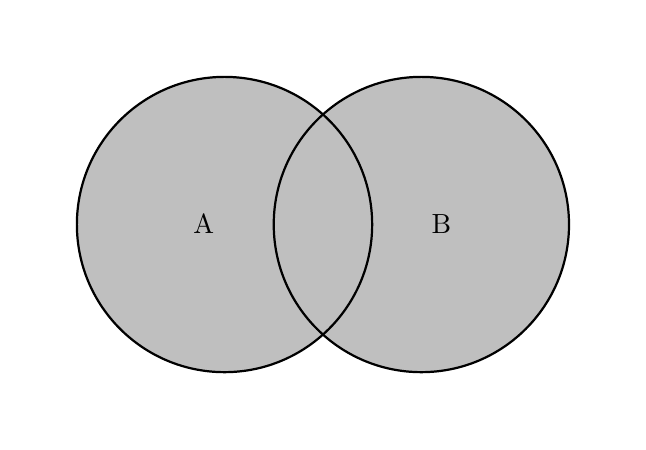
\begin{tikzpicture}[thick,scale=1.25]
\fill[white] (-2,-2) -- (4,-2) -- (4,2) -- (-2,2) -- cycle;
\fill[lightgray] (0,0) circle (1.5cm);
\fill[lightgray] (2,0) circle (1.5cm);
\draw (0,0) circle (1.5cm) node[left] {A};
\draw (2,0) circle (1.5cm) node[right] {B};
\end{tikzpicture}


\textbf{\large Intersection}

$P\cap Q$

All elements in both $P$ \textit{and} $Q$

\bigskip
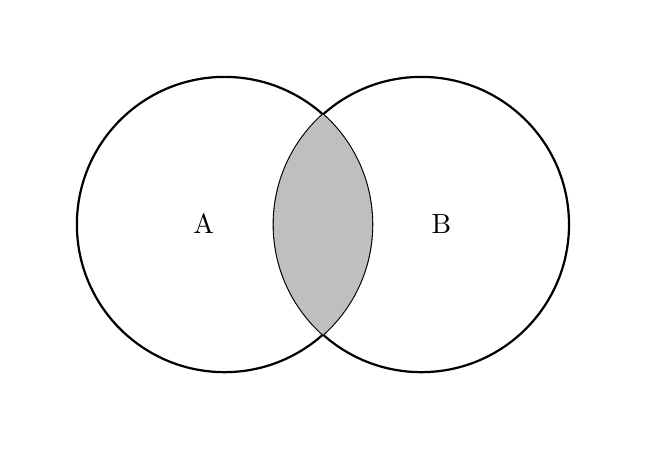
\begin{tikzpicture}[thick,scale=1.25]
\fill[white] (-2,-2) -- (4,-2) -- (4,2) -- (-2,2) -- cycle;
\draw (0,0) circle (1.5cm) node[left] {A};
\draw (2,0) circle (1.5cm) node[right] {B};
\clip (0,0) circle (1.5cm);
\fill[lightgray] (2,0) circle (1.5cm);
\end{tikzpicture}
\end{multicols}
\end{center}
\end{equationbox}

\bigskip
\begin{enumerate}[labelindent=*,style=multiline,leftmargin=*,label=\textbf{Example \arabic*:}]
\item Martha's has 15 cupcakes that are vanilla frosted and 10 cupcakes that are chocolate frosted. If two-thirds of Martha's cupcakes are both vanilla and chocolate frosted, how many cupcakes have vanilla frosting?
\vfill\item In the set of integers from 1 to 100 inclusively, how many numbers are divisible by 3 or 5 but not both?
\vfill\item Mr. Dropal has 16 students in his class. There are 10 male students. Half of all students are taking only Chinese and one-quarter are taking Chinese and French. If the class must take either French or Chinese, what proportion represents the maximum number of females taking only French?
\end{enumerate}

\vfill
\newpage
\begin{multicols*}{2}
\begin{outline}[enumerate]
\medium

\1 Mr. Carter has a garden of yellow, white, and red rose bushes. The proportion of red rose bushes to all other bushes is 0.4. When he buys an additional 4 red rose bushes, the proportion increases to 0.5. How many non-red rose bushes did Mr. Carter originally have?

\bigskip
\textbf{Equation/Strategy:} \hrulefill

\bigskip
\textbf{Solve:}

\vfill
\2 8
\2 12
\2 20
\2 24
\2 36

\midline

\1 The average (arithmetic mean) of a set of 5 positive integers is 10 and the median is 10. What is the largest possible value of the largest member of the set?

\bigskip
\textbf{Equation/Strategy:} \hrulefill

\bigskip
\textbf{Solve:}

\vfill
\2 10
\2 50
\2 22
\2 37
\2 40

\columnbreak
\advanced

\1 Helen has a box of 40 chocolates. The proportion cherry filled or coconut chocolates is 0.3, whereas the proportion of coconut or creme filled is 0.4. If the number of creme filled is twice the number of cherry filled and there is at least one cherry filled, what proportion of the box is coconut?

\bigskip
\textbf{Equation/Strategy:} \hrulefill

\bigskip
\textbf{Solve:}

\vfill
\2 0.075
\2 0.1
\2 0.15
\2 0.2
\2 0.25

\midline

\1 When a positive integer $n$ is divided by 4, the remainder is 3. When $n$ is divided by 5, the remainder is 1. How many values of $n$ are there from 1 to 40?

\bigskip
\textbf{Equation/Strategy:} \hrulefill

\bigskip
\textbf{Solve:}

\vfill
\2 0
\2 1
\2 2
\2 3
\2 4
\end{outline}
\end{multicols*}